\documentclass[a4paper,14pt]{article}

\usepackage{comment} % Para comentar várias linhas ao mesmo tempo

%matemática
\usepackage{amsmath}
\usepackage{amssymb}

%diagramação
\usepackage{extsizes}
\everymath{\displaystyle}
\usepackage{geometry}
\usepackage{fancyhdr}
\usepackage{multicol}
\usepackage{graphicx}
\usepackage[brazil]{babel}
\usepackage[shortlabels]{enumitem}
\usepackage{cancel}
\usepackage{textcomp}
\usepackage{tcolorbox}

%tabelas
\usepackage{array} % Para melhor formatação de tabelas
\usepackage{longtable}
\usepackage{booktabs}  % Para linhas horizontais mais bonitas
\usepackage{float}   % Para usar o modificador [H]
\usepackage{caption} % Para usar legendas em tabelas
\usepackage{wrapfig} % Para usar tabelas e figuras flutuantes


%tikzpicture
\begin{comment}
	\usepackage{tikz}
	\usepackage{scalerel}
	\usepackage{pict2e}
	\usepackage{tkz-euclide}
	\usetikzlibrary{calc}
	\usetikzlibrary{patterns,arrows.meta}
	\usetikzlibrary{shadows}
	\usetikzlibrary{external}
\end{comment}


%pgfplots
\usepackage{pgfplots}
\pgfplotsset{compat=newest}
\usepgfplotslibrary{statistics}
\usepgfplotslibrary{fillbetween}

%colours
\usepackage{xcolor}



\columnsep=2cm
\hoffset=0cm
\textwidth=8cm
\setlength{\columnseprule}{.1pt}
\setlength{\columnsep}{2cm}
\renewcommand{\headrulewidth}{0pt}
\geometry{top=1in, bottom=1in, left=0.7in, right=0.5in}

\pagestyle{fancy}
\fancyhf{}
\fancyfoot[C]{\thepage}

\begin{document}
	
	\noindent\textbf{6FMA15 - Matemática} 
	
	\begin{center}Sistemas de numeração (Versão estudante)
	\end{center}
	
	\noindent\textbf{Nome:} \underline{\hspace{10cm}}
	\noindent\textbf{Data:} \underline{\hspace{4cm}}
	
	%\section*{Questões de Matemática}
	
	\begin{multicols}{2}
		\noindent O sistema de numeração decimal é usado no mundo inteiro atualmente. A multiplicação de um número $a$ por ele mesmo, $n$ vezes, é representada por $a^n$, que chamamos de potência de base $a$ e expoente $n$. \\
		No sistema de numeração romana são usados apenas sete algarismos para representar os números: I, V, X, L, C, D e M, que correspondem, respectivamente, aos numerais indo-arábicos 1, 5, 10, 50, 100, 500 e 1 000. \\
		\noindent\textsubscript{-----------------------------------------------------------------------}
		\begin{enumerate} 
			\item Diga qual a posição do algarismo 8 e seu expoente correspondente.
			\begin{enumerate}[a)]
				\item 3 472 103 824 \\\\\\\\
				\item 541 810 352 \\\\\\\\
				\item 129 567 281 \\\\\\\\
				\item 28 376 410 \\\\
			\end{enumerate}
			\item Escreva o numeral que representa:
			\begin{enumerate}[a)]
				\item $6 \cdot 10^5 + 5 \cdot 10^4 + 2 \cdot 10^3 + 1 \cdot 10 + 3$ \\\\\\\\
				\item $2 \cdot 10^4 + 7 \cdot 10^2 + 6 \cdot 10 + 4$ \\\\\\\\
				\item $7 \cdot 10^7 + 1 \cdot 10^4 + 2 \cdot 10^3 + 3 \cdot 10^2 + 5$ \\\\\\\\
				\item $3 \cdot 10^5 + 2 \cdot 10^3 + 8$ \\\\\\\\
			\end{enumerate}
			\item Dado o número na forma de potência $5^4$:
			\begin{enumerate}[a)]
				\item diga qual é a base e qual é o expoente.  \newpage
				\item diga se o seu valor é maior ou menor do que 1 000. \\\\\\\\
			\end{enumerate}
			\item Represente simplificadamente.
			\begin{enumerate}[a)]
				\item $10 \cdot 10 \cdot 10 \cdot 10 \cdot 10 \cdot 10 \cdot 10$ \\\\\\\\
				\item $\underbrace{10 \cdot 10 \cdot ... \cdot 10}$ \\ $.~~~12$ vezes \\\\\\\\
			\end{enumerate}
			\item Usando algarismos romanos, escreva os números de 1 a 25. \\\\\\\\\\\\\\\\\\\\
			\item Qual número é maior: MDLX ou MDXXXVIII?  \\\\\\\\\\\\
			\item Escreva os numerais representados pelas expressões:
			\begin{enumerate}[a)]
				\item $5 \cdot 10^4 + 8 \cdot 10^2 + 7$ \\\\\\\\\\
				\item $3 \cdot 10^3 + 2 \cdot 10^2 + 1$ \\\\\\\\\\
				\item $4 \cdot 10^5 + 8 \cdot 10^4 + 7 \cdot 10^2 + 5 \cdot 10 + 2$ \\\\\\\\\\
				\item $7 \cdot 10^5 + 4 \cdot 10^3 + 8 \cdot 10^2 + 3$ \\\\\\\\\\
				\item $9 \cdot 10^9 + 7 \cdot 10^6 + 5$ \\\\\\\\\\
				\item $2 \cdot 10^5 + 10^4 + 10^3 + 10^2 + 10$ \\\\\\\\\\\\
			\end{enumerate}
			\item Diga quantos algarismos tem o número:
			\begin{enumerate}[a)]
				\item $7 \cdot 10^12 + 3$ \\\\\\\\\\
				\item $5 \cdot 10^{15} + 8$ \\\\\\\\\\
				\item $60 \cdot 10^{30} + 1$ \\\\\\\\\\
				\item $276 \cdot 10^{80} + 1$ \\\\\\\\\\
				\item $2 137 \cdot 10^{62} + 4$ \\\\\\\\\\
				\item $102 \cdot 10^{100} + 3$ \\\\\\\\\\
			\end{enumerate}
			\item Escreva usando algarismo romanos:
			\begin{enumerate}[a)]
				\item 526 \\\\\\
				\item 1 999 \\\\\\
				\item 3 200 \\\\\\
				\item 1 940 \\\\\\
				\item 1 637 \\\\\\
				\item 372 \\\\\\
			\end{enumerate}
			\item Os egípcios usavam um sistema similar ao sistema romano, porém com menos símbolos. Uma exceção é o fato de os egípcios terem um símbolo para um milhão, um homem com os braços levantados. Os romanos não tinham um símbolo equivalente. \\
			A figura abaixo compara os dois sistemas. \\
			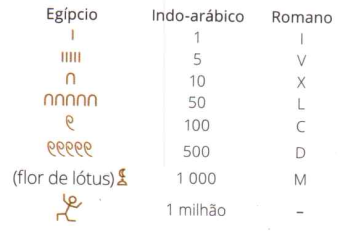
\includegraphics[width=1.1\linewidth]{6FMA15_imagens/imagem1}
			\begin{enumerate}[a)]
				\item Escreva o número 4 274 nos dois sistemas. \\\\\\\\
				\item Converta o número MCMLXXXIV para o sistema egípcio. \\\\\\\\
			\end{enumerate}
			\item (ENEM) Os maias desenvolveram um sistema de numeração vigesimal que podia representar qualquer número inteiro, não negativo, com apenas três símbolos. Uma concha representava o zero, um ponto representava o número 1 e uma barrinha horizontal, o número 5. Até o número 19 os maias representavam os números como mostra a figura 1: \\
			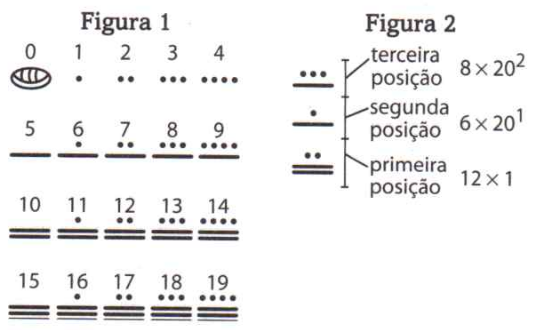
\includegraphics[width=1.1\linewidth]{6FMA15_imagens/imagem2} \\
			Números superiores a 19 são escritos na vertical, seguindo potências de 10 em notação posicional, como mostra a figura 2. \\
			Ou seja, o número que se encontra na primeira posição é multiplicado por $20^0 = 1$, o número que se encontra na segunda posição é multiplicado por $20^1 = 20$ e assim por diante. Os resultados obtidos em cada posição são somados para obter o número no sistema decimal. \\
			Um arqueólogo achou o hieróglifo da figura 3 em um sítio arqueológico: \\
			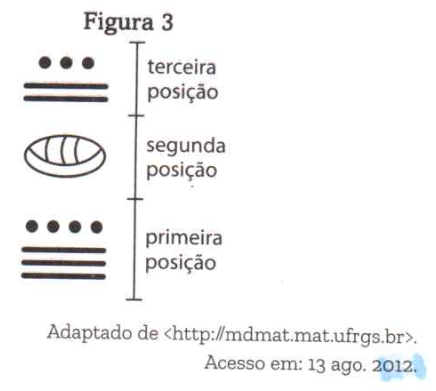
\includegraphics[width=1.1\linewidth]{6FMA15_imagens/imagem3} \\
			O número, no sistema decimal, que o hieroglifo da figura 3 representa é igual a:
			\begin{enumerate}[a)]
				\item 279
				\item 539
				\item 2 619
				\item 5 219
				\item 7 613
			\end{enumerate}
		\end{enumerate}
		$~$ \\ $~$ \\ $~$ \\ $~$ \\ $~$ \\ $~$ \\ $~$ \\ $~$ \\ $~$ \\ $~$ \\ $~$ \\ $~$ \\ $~$ \\ $~$ \\ $~$ \\ $~$ \\ $~$ \\ $~$ \\ $~$ \\ $~$ \\ $~$ \\ $~$ \\ $~$ \\ $~$ \\ $~$ \\ $~$ \\ $~$ \\ $~$ \\ $~$ \\ $~$ \\ $~$ \\ $~$ \\ $~$ \\ $~$ \\ $~$ \\ $~$ \\ $~$ \\ $~$ \\ $~$ \\ $~$ \\ $~$ \\ $~$ \\ $~$ \\ $~$ \\ $~$ \\ $~$ \\ $~$ \\ $~$ \\ $~$ \\ $~$ \\ $~$ \\ $~$ \\ $~$ \\ $~$ \\ $~$ \\ $~$ \\ $~$ \\ $~$ \\ $~$ \\ $~$ \\ $~$ \\ $~$ \\ $~$ \\ $~$ \\ $~$ \\ $~$ \\ $~$ \\ $~$ \\ $~$ \\ $~$ \\ $~$ \\ $~$ \\ $~$ \\ $~$ \\ $~$ \\ $~$ \\ $~$ \\ 
	\end{multicols}
\end{document}